\documentclass[a4paper,12pt]{report}
\include{basic}
\usetikzlibrary {arrows.meta}
\usetikzlibrary{external}
\tikzexternalize[prefix=./] %  your external folderName= build
\usetikzlibrary{calc}



\pgfplotsset{compat=1.15}
\def\title{BAK - Bakalářská práce}
\def\subtitle{poznámky}
\def\author{Havránek Kryštof}
\def\institution{ČVUT FEL - EK}
\def\supervisor{Ing. Viktor Adler Ph.D.}

\include{makra}
\include{notes}

\begin{document}

\titlep
\tocp

\pagestyle{plain}
\pagenumbering{arabic}

\chapter{FMCW radary}

\begin{itemize}
	\item CW - continuous wave
		\begin{itemize}
			\item transmits a continuous wave on a single frequency
			\item detects targets via a harmonic beat signal with a Doppler frequency of $f_D = \frac{2v_r}{\lambda_c} = \frac{2v_r f_c}{c_0}$ where $\lambda_c/f_c$ is the wavelength or frequency of the transmitted signal
			\item only information about presence of the target and his radial velocity (part of velocity vector that is pointing towards source of signal) can be gathered
		\end{itemize}
	\item FMCW - frequency modulated continuous wave
		\begin{itemize}
			\item transmits a continuous wave with a frequency that is modulated by a linear function (frequency periodically increases or decreases)
			\item one frequency sweep is called a chirp/frame
			\item detects round-trip delay vai frequency of a beat signal
			\item received power is determined by radar equation
				\[
					P_r = \frac{P_t G_t G_r \lambda^2 \sigma}{(4\pi)^3 R^4}
				\]
				where $\sigma$ is the radar cross section of the target, $\lambda$ is the wavelength of the transmitted signal, $R$ is the distance to the target, $P_t$ is the transmitted power, $G_t$ is the gain of the transmitting antenna, $G_r$ is the gain of the receiving antenna
			\item achievable radar parameters
				\begin{center}
					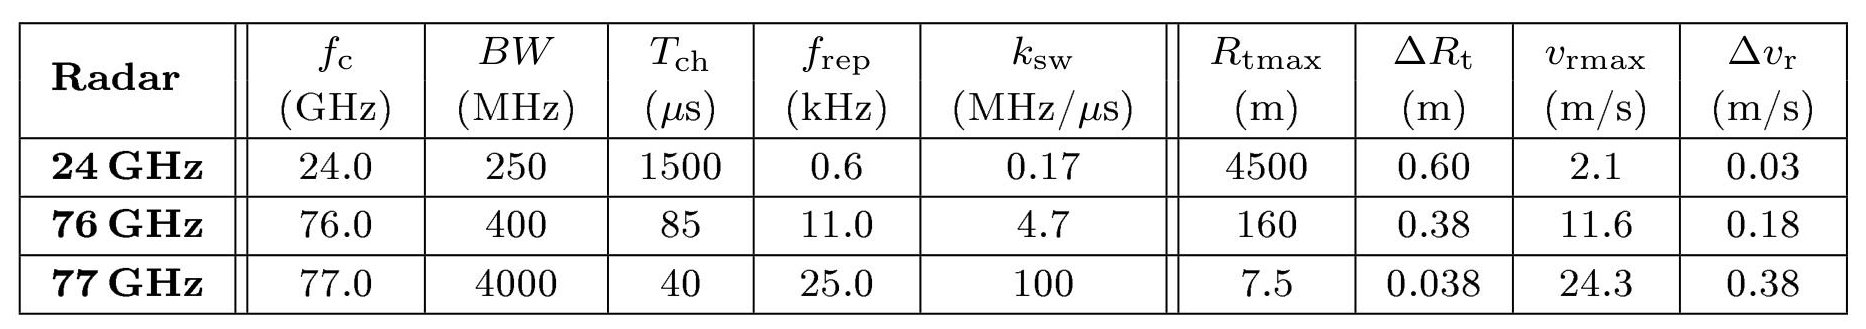
\includegraphics[width=0.8\textwidth]{./img/fmcw_radar_paramters.jpg}
				\end{center}
		\end{itemize}
	\item transmitted signal
		\begin{center}
			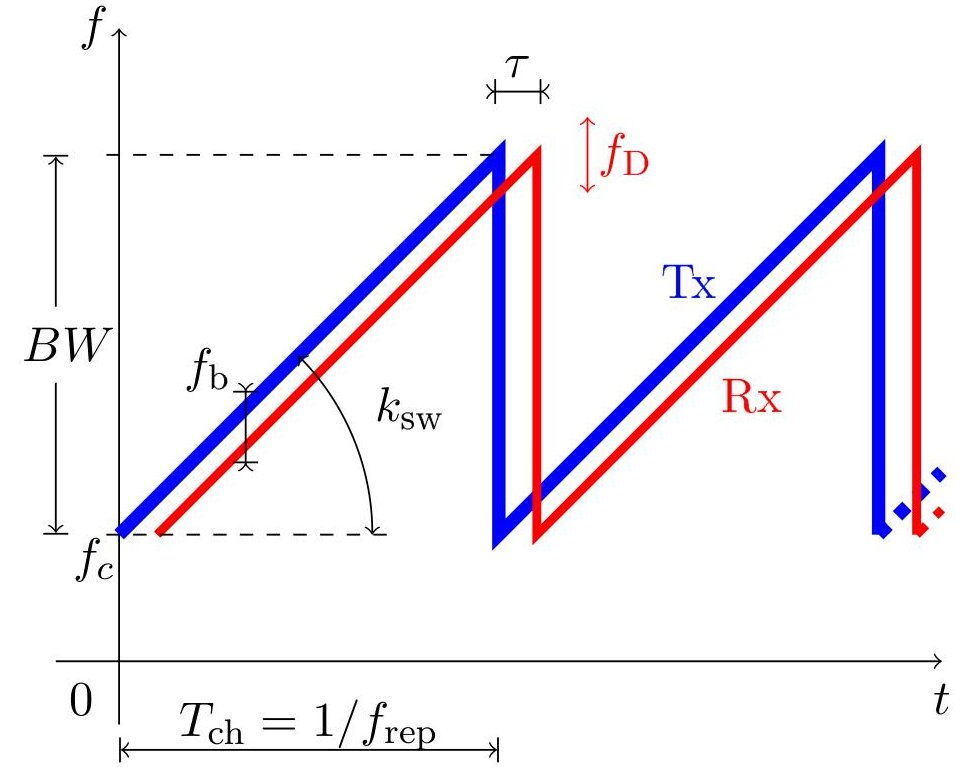
\includegraphics[width=0.4\textwidth]{./img/fmcw_signal_ft_relation.jpg}
		\end{center}
		\begin{itemize}
			\item $\tau$ -- time delay between transmitted signal on $T_X$ and received signal on $R_X$
			\item $f_c$ -- carrier frequency that is modulated, usually in tens of GHz
			\item $BW$  -- bandwidth of the chirp, from roughly 100MHz to 6GHz
			\item $T_{ch}$ -- duration of the chirp
			\item $k_{sw} = T_{ch}/BW$ -- chirp slope (how fast we sweep the frequency across the bandwidth)
			\item $f_D$ -- Doppler frequency of moving target
			\item form of a real transmitted signal
				\begin{center}
					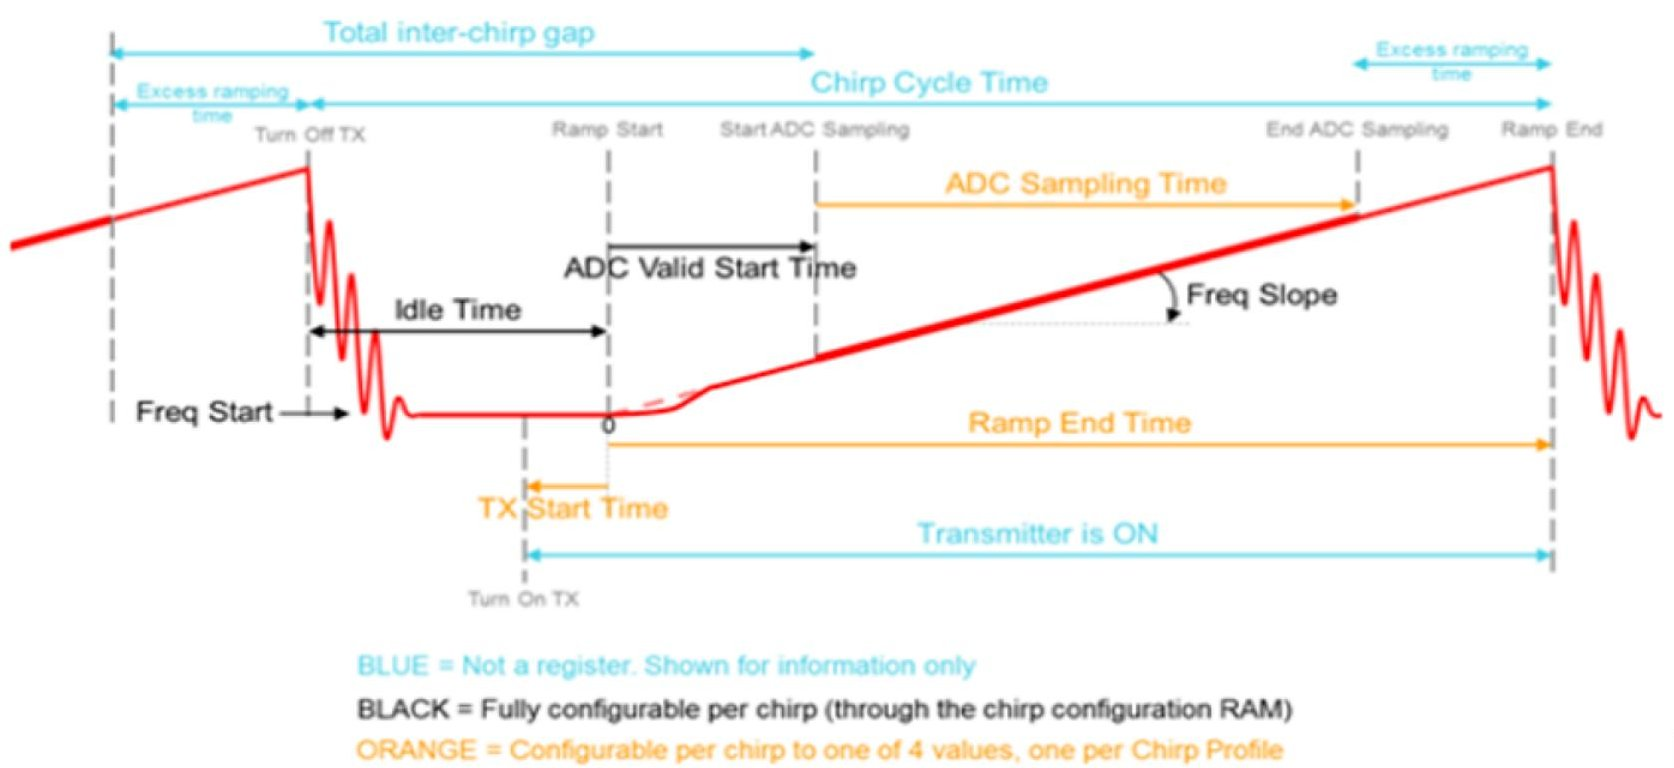
\includegraphics[width=0.7\textwidth]{./img/fmcw_chirp_shape.jpg}
				\end{center}
		\end{itemize}
	\item beat signal
		\begin{itemize}
			\item in FMCW radars we use so called filtered harmonic beat that is defined as $f_{beat}(t) = f_{Tx}(t)f_{Rx}(t)$
			\item transmitted signal is changing its frequency within the chirp as $f_{Tx}(t) = f_c + k_{sw}t$, thus it transcription can be written as $s_{Tx}(t)= A_c \cos(2\pi f_c t + \pi k_{sw} t^2)$
			\item signal on receiver is delayed by $\tau$ thus $s_{Rx}(t) = s_{Tx}(t-\tau) = A_c \cos(2\pi f_c (t-\tau) + \pi k_{sw} (t-\tau)^2)$
			\item combining these two signals in a mixer we get our output
				\[
					s_{out}(t) = \frac{A_c^2}{2} (\cos((2\omega_c - 2\pi k_{sw}\tau )t + 2\pi k_{sw}t^2 + (\pi k_{sw} \tau^2 - \omega_c\tau)) \times \cos(2\pi k_{sw} \tau t + (\omega_c \tau - \pi k_{sw} \tau^2) ))
				\]
				\begin{itemize}
					\item first cosine term describes a linearly increasing FM signal at roughly twice the carrier frequency  with a phase shift that is proportional to the delay $\tau$
					\item generally no usefully information can be gathered from the first term and is usually filtered out, that can be done simply with a low-pass filter given its higher frequency
					\item second cosine term describes a beat signal at a fixed frequency that can be calculated with derivation of the phase shift
						\[
							f_b = \frac{1}{2\pi} \frac{d }{d t} (2\pi k_{sw}\tau t + (\omega_c \tau + \pi k_{sw} \tau^2)) = k_{sw}\tau
						\]
					\item we can see that the frequency is proportional to the delay and chirp slope
				\end{itemize}
		\end{itemize}
	\item estimating range with a FMCW radar
		\begin{itemize}
			\item relation between beat signal frequency and distance can be derived as $f_{beat} = \frac{2R_t}{c_0} \frac{BW}{T_{ch}} = \tau k_{sv}$
			\item for signal transmitted in air ve can defined relation $\tau = \frac{2R}{c}$ $\Rightarrow$ $f_b = k_{sw} \frac{2R}{c} $
			\item thus we can estimate the range as
				\[
					R_t = \frac{f_b c_0}{2k_{sw}}
				\]
			\item in real applications maximal beat frequency detectable is determined by the sampling frequency we use
				\[
					f_{beat, max} = f_{s}/2
				\]
				\begin{itemize}
					\item between number of samples and sampling frequency there is relation $N_s = T_{ch} f_s$
					\item ideally we have at least $N_s+1$ samples
					\item we can use both real or IQ sampling
					\item negative frequencies enables us to do a estimation of noise flow
				\end{itemize}
				% \item maximal detectable range is given predominantly by the chirp length -- $R_{t, max} = \frac{f_s c_0}{4k_{sw}} $
			\item FT of the beat signal returns $N_s$-sample complex frequency spectrum with width of $f_s$, that gives us a resolution of $\delta f_b = f_s/N_s \sim \frac{1}{T_{ch}}$
				\begin{itemize}
					\item to get a range resolution we can easily substitute frequency with frequency resolution
						\[
							\delta R = \frac{c_0 k_{sw}}{2} \delta f_b \sim \frac{c_0}{2BW}
						\]
					\item we can see that range resolution is determined by the bandwidth and does not depend on the sampling frequency
					\item unfortunately given dependence  on $k_{sw}$ if the chirp slope is not linear then the range resolution will not be constant (degrades with a derivation of the chirp slope)
				\end{itemize}
			\item improving the range resolution
				\begin{itemize}
					\item most often resolution can be improved by linearsing the chirp slope most often done with a pre-programmed look up table
					\item however more complicated circuits (most notably delay-line discriminator) can also be used to achieve the same effect
					\item often superposition of neighboring chirps is also used to increase the resolution
				\end{itemize}
			\item effect of transmitted signal reaching the receiver via the PCB
				\begin{itemize}
					\item single antenna or event a dual antenna configuration results in a significant power leaking into the receiver
					\item as we are transmitting and receiving at the same time this poses a significant problem
					\item this noise must be mitigated primarly with physical design of the radar otherwise if the leakage signal is too high it cal bias the mixer resulting in a significant error
				\end{itemize}
			\item effects of phase noise
				\begin{itemize}
					\item any transmitter will exhibit a certain amount of phase noise, that can be added to our $s_{out}$ equation in following way
						\[
							s_{out}(t) = \frac{A_c^2}{2} (\cos(2\pi k_{sw} \tau t + (\omega_c \tau - \pi k_{sw} \tau^2)+\phi(t) + \phi(t) - \phi(t-\tau))
						\]
				\end{itemize}
		\end{itemize}
	\item estimating speed with FMCW radar
		\begin{itemize}
			\item it is impossible to determine speed of the target from a single chirp
			\item estimation of speed is not as precise as estimation of range
			\item to get any useful estimation $\frac{2R_t k_{sw}}{c_0} \gg \frac{2v_r f_c}{c_0}$
			\item doppler shift causes as phase shift in the beat signal
			\item to get estimation of $f_D$ we rely on FT of the beat signals
			\item speed resolution $\Delta v_t = \frac{c_0}{2T_{ch}N_{ch}f_c} $
			\item speed limit $v_{r,max} = \pm \frac{f_{rep} c_0}{4f_c}$ where $f_{rep} = \frac{1}{T_{ch}}$ and $f_{d, max}= \pm \frac{f_{rep}}{2} $
		\end{itemize}
\end{itemize}

\end{document}
